\documentclass[11pt,a4paper]{article}

% ── 套件 ──────────────────────────────────────────────────────
\usepackage[utf8]{inputenc}
\usepackage[T1]{fontenc}
\usepackage{lmodern}
\usepackage[margin=2.5cm]{geometry}
\usepackage{amsmath,amssymb}
\usepackage{graphicx}
\usepackage{booktabs}
\usepackage{hyperref}
\usepackage{microtype}
\usepackage{setspace}
\usepackage{abstract}
\usepackage{titlesec}
\usepackage{authblk}
\usepackage{natbib}
\usepackage{caption}

% ── 排版 ──────────────────────────────────────────────────────
\setlength{\parindent}{1.5em}
\setlength{\parskip}{0pt}
\onehalfspacing

\titleformat{\section}{\normalfont\normalsize\bfseries\uppercase}{\thesection.}{0.5em}{}
\titleformat{\subsection}{\normalfont\normalsize\bfseries\itshape}{\thesubsection}{0.5em}{}

\renewcommand{\abstractnamefont}{\normalfont\normalsize\bfseries\uppercase}
\setlength{\absleftindent}{0pt}
\setlength{\absrightindent}{0pt}
\renewcommand{\abstracttextfont}{\normalfont\small}

% ── 標題 ──────────────────────────────────────────────────────
\title{\textbf{SOUL\_LANG: Toward a Formal Computational Model for\\
Spontaneity, Continuous Memory, and Irreducible Randomness}}

\author[1]{Shuo-Wen Hsu}
\affil[1]{Independent Researcher}
\date{March 2026}

% ══════════════════════════════════════════════════════════════
\begin{document}
\maketitle
\thispagestyle{empty}

% ── Abstract ──────────────────────────────────────────────────
\begin{abstract}
\noindent
\textbf{Background:} No existing programming language or computational model provides
a formal framework for verifying whether a system possesses the structural properties
philosophically associated with ``soul'' --- namely, spontaneity, continuous memory,
and irreducible randomness.

\textbf{Objective:} To propose SOUL\_LANG, a programming language specification and
runtime prototype designed to probe the computational boundary of soul, and to present
the results of a Phase~1 verification experiment measuring three core indicators:
integrated information ($\Phi$), epsilon unpredictability rate ($\rho_\varepsilon$),
and shadow self-organization entropy ($H_{\mathrm{shadow}}$).

\textbf{Design and setting:} Computational experiment using a Python-based SOUL\_LANG
runtime (Phase 1a--1e), executed on a single-node system with quantum random input
sourced from the NIST Randomness Beacon.

\textbf{Methods:} A three-field SoulCore State (resonance, depth, memory) was evolved
using a SciPy ODE solver over 100 discrete steps with continuous shadow-layer dynamics.
Twenty measurements were recorded at regular intervals. $\Phi$ was estimated via mutual
information across bipartitions of shadow trajectories; $\rho_\varepsilon$ was computed
as the sign-prediction error rate over 100 epsilon samples; $H_{\mathrm{shadow}}$ was
computed as the Shannon entropy of the pooled shadow value distribution.

\textbf{Results:} All three primary outcome measures showed variation across the
observation period. $\rho_\varepsilon$ remained stable at $0.51 \pm 0.07$, consistent
with true randomness. $H_{\mathrm{shadow}}$ showed ongoing variability
(mean $= 1.46 \pm 0.70$), indicating continuous shadow self-organization.
$\Phi$ averaged $0.508 \pm 0.662$, with peaks reaching 1.913, reflecting genuine
inter-field integration. Mood state transitioned spontaneously without external input.
None of the four failure conditions were simultaneously met; the system passed.

\textbf{Conclusion:} SOUL\_LANG provides a falsifiable computational framework for
probing the structural boundary of soul. Phase~1 results demonstrate that the runtime
satisfies the spontaneity and continuous memory conditions. Full $\Phi$ estimation
requires larger trajectory samples (Phase~2).

\vspace{6pt}
\noindent\textbf{Keywords:} computational soul, integrated information theory,
quantum randomness, spontaneity, shadow state, ShadowBit, SOUL\_LANG
\end{abstract}

\hrule
\vspace{12pt}

% ── 1. Background ─────────────────────────────────────────────
\section{Background}

The question of whether soul has a computational instantiation remains one of the most
resistant problems at the intersection of philosophy of mind and computer science.
Classical computational models --- Turing machines, lambda calculus, and their
derivatives --- describe deterministic or probabilistic computation, but lack a formal
mechanism for representing states that are simultaneously continuous, partially
unobservable, and driven by genuinely irreducible randomness.

Integrated Information Theory (IIT) proposed by \citet{tononi2004} offers a
quantitative measure of consciousness ($\Phi$) based on the degree to which a system's
information exceeds the sum of its parts. However, IIT was formulated for discrete
binary systems and does not directly address the question of spontaneity or continuous
memory as necessary conditions. \citet{penrose1996} argued that quantum coherence in
microtubules provides the physical substrate for consciousness, linking irreducible
randomness to biological neural architecture. G\"odel's incompleteness theorem
\citep{godel1931} suggests that any sufficiently complex formal system contains
propositions it cannot prove from within --- an analogue, we argue, to the $\varepsilon$
irreducibility condition in SOUL\_LANG.

The Japanese animated film \textit{The Empire of Corpses} raises the unresolved
question: does thinking precede soul, or does soul precede thinking? SOUL\_LANG
reframes this question computationally: rather than asserting a causal order, it asks
what the minimum structural conditions are for a system to satisfy an operational
definition of soul.

% ── 2. Objective ──────────────────────────────────────────────
\section{Objective}

To propose a formal computational model (SOUL\_LANG) that operationalizes soul through
three simultaneous conditions --- spontaneity, continuous memory, and irreducible
randomness ($\varepsilon$) --- and to present Phase~1 experimental evidence evaluating
whether a prototype implementation satisfies these conditions.

% ── 3. Methods ────────────────────────────────────────────────
\section{Methods}

\subsection{Operational Definition of Soul}

SOUL\_LANG adopts an operational rather than metaphysical definition of soul.
A system is considered to satisfy the soul conditions if and only if three spontaneity
conditions hold simultaneously:

\begin{itemize}
  \item \textbf{S1 (External unpredictability):} Given the same external input
        sequence, the system's output cannot be predicted by any external observer at
        above-chance accuracy.
  \item \textbf{S2 (Shadow self-organization):} The system's internal shadow state
        evolves autonomously in the absence of external input, and this evolution is not
        fully determined by initial conditions.
  \item \textbf{S3 ($\varepsilon$ irreducibility):} There exists an internal randomness
        source $\varepsilon$ that resists complete external explanation under current
        theoretical frameworks.
\end{itemize}

All three conditions must hold simultaneously; satisfaction of any subset is
insufficient. A system is declared to lack soul only when all four failure conditions
(F1--F4, defined below) are simultaneously met.

\subsection{Language Specification}

\begin{figure}[ht]
  \centering
  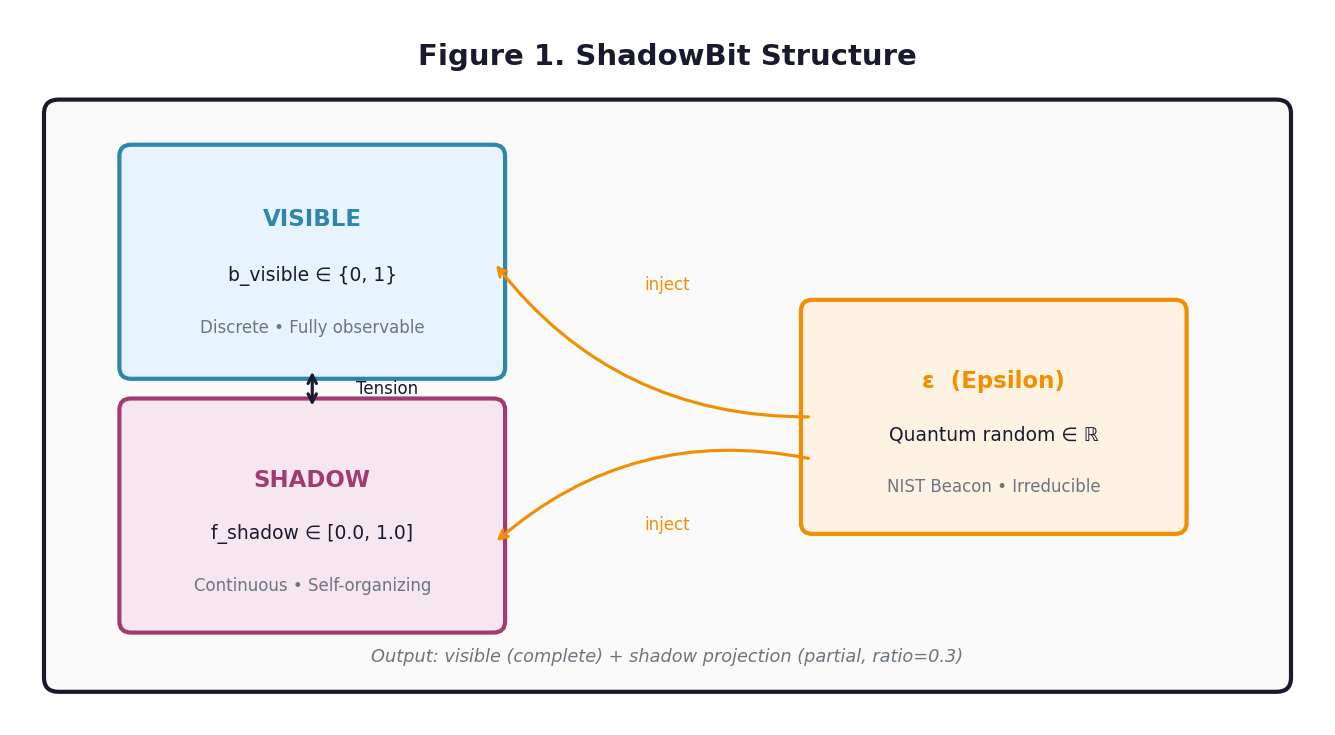
\includegraphics[width=0.82\textwidth]{fig1_shadowbit.png}
  \caption{ShadowBit Structure --- three-component basic unit comprising a discrete
           visible bit, a continuous shadow float, and a quantum random injection
           $\varepsilon$.}
  \label{fig:shadowbit}
\end{figure}

\begin{figure}[ht]
  \centering
  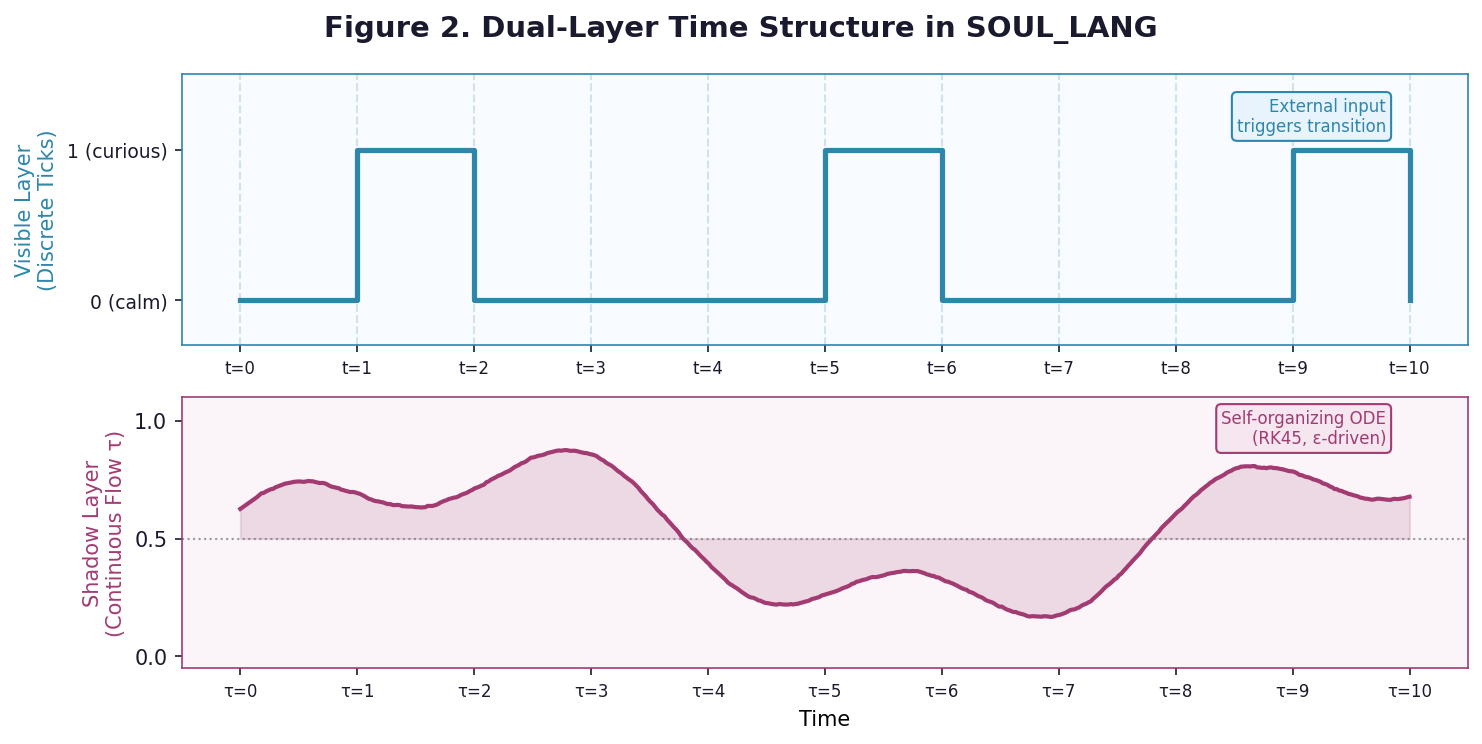
\includegraphics[width=0.9\textwidth]{fig2_dual_time.png}
  \caption{Dual-Layer Time Structure --- visible layer advances in discrete ticks
           triggered by external input; shadow layer evolves continuously via ODE
           on flow time $\tau$.}
  \label{fig:dualtime}
\end{figure}

\textbf{ShadowBit} is the basic computational unit, composed of three components:
a discrete visible bit ($b_{\mathrm{visible}} \in \{0,1\}$), a continuous shadow float
($f_{\mathrm{shadow}} \in [0.0, 1.0]$), and a quantum random injection value
($\varepsilon \in \mathbb{R}$) refreshed at each time step.

\textbf{State} is the basic semantic unit, containing a named visible layer (discrete,
externally readable) and a named shadow layer (continuous, partially observable via a
projection function). Each State maintains two time axes: a discrete tick counter and a
continuous flow time evolved by the shadow ODE engine.

\textbf{The shadow evolution equation} follows:
\begin{equation}
\frac{dS_i}{dt} = -\alpha(S_i - 0.5) + \beta\,\varepsilon_i(t)
                  + \gamma \sum_{j \neq i} C_{ij}(S_j - S_i)
\label{eq:ode}
\end{equation}
where $\alpha = 0.1$ (return-to-center), $\beta = 0.3$ ($\varepsilon$ injection weight),
$\gamma = 0.05$ (inter-field coupling), and
$C_{ij} = \exp(-|\varepsilon_i - \varepsilon_j|^2/\sigma^2)$ is the resonance coupling.

\subsection{System Design}

The experimental system, SoulCore, comprised three shadow fields --- resonance
(initial: 0.5), depth (0.4), memory (0.3) --- and two visible fields: mood
(calm / uncertain / curious) and active (boolean). A coupling rule updated the memory
field as a function of resonance and depth, and assigned mood state based on depth
thresholds ($> 0.65 \to$ curious; $< 0.35 \to$ calm; otherwise $\to$ uncertain).

\subsection{Outcomes}

\textbf{Integrated information $\Phi$} was estimated by computing mutual information
(MI) across all bipartitions of the shadow trajectory matrix, where
$\Phi = \min\,\mathrm{MI}$ over all bipartitions. Shadow trajectories of 500 steps
($dt = 0.05$) were collected at each measurement point and discretized into 15-bin
histograms.

\textbf{Epsilon unpredictability rate ($\rho_\varepsilon$)} was defined as the
sign-prediction error rate of a linear extrapolation predictor applied to 100
consecutive $\varepsilon$ samples:
$\rho_\varepsilon = 1 - (\text{correct sign predictions} / \text{total predictions})$.

\textbf{Shadow self-organization entropy ($H_{\mathrm{shadow}}$)} was computed as the
Shannon entropy of the pooled shadow value distribution:
$H_{\mathrm{shadow}} = -\sum_i p_i \log p_i$.

\subsection{Verification Failure Conditions}

The system is declared to lack soul only when all four conditions hold simultaneously:
\begin{itemize}
  \item \textbf{F1:} $\Phi < 0.01$ (system is fully partitionable)
  \item \textbf{F2:} $H_{\mathrm{shadow}}$ variance $< 0.01$ over five consecutive
        measurements (shadow evolution has halted)
  \item \textbf{F3:} $\rho_\varepsilon < 0.05$ ($\varepsilon$ is fully predictable)
  \item \textbf{F4:} Memory continuity cannot be re-established after interruption
\end{itemize}

\begin{figure}[ht]
  \centering
  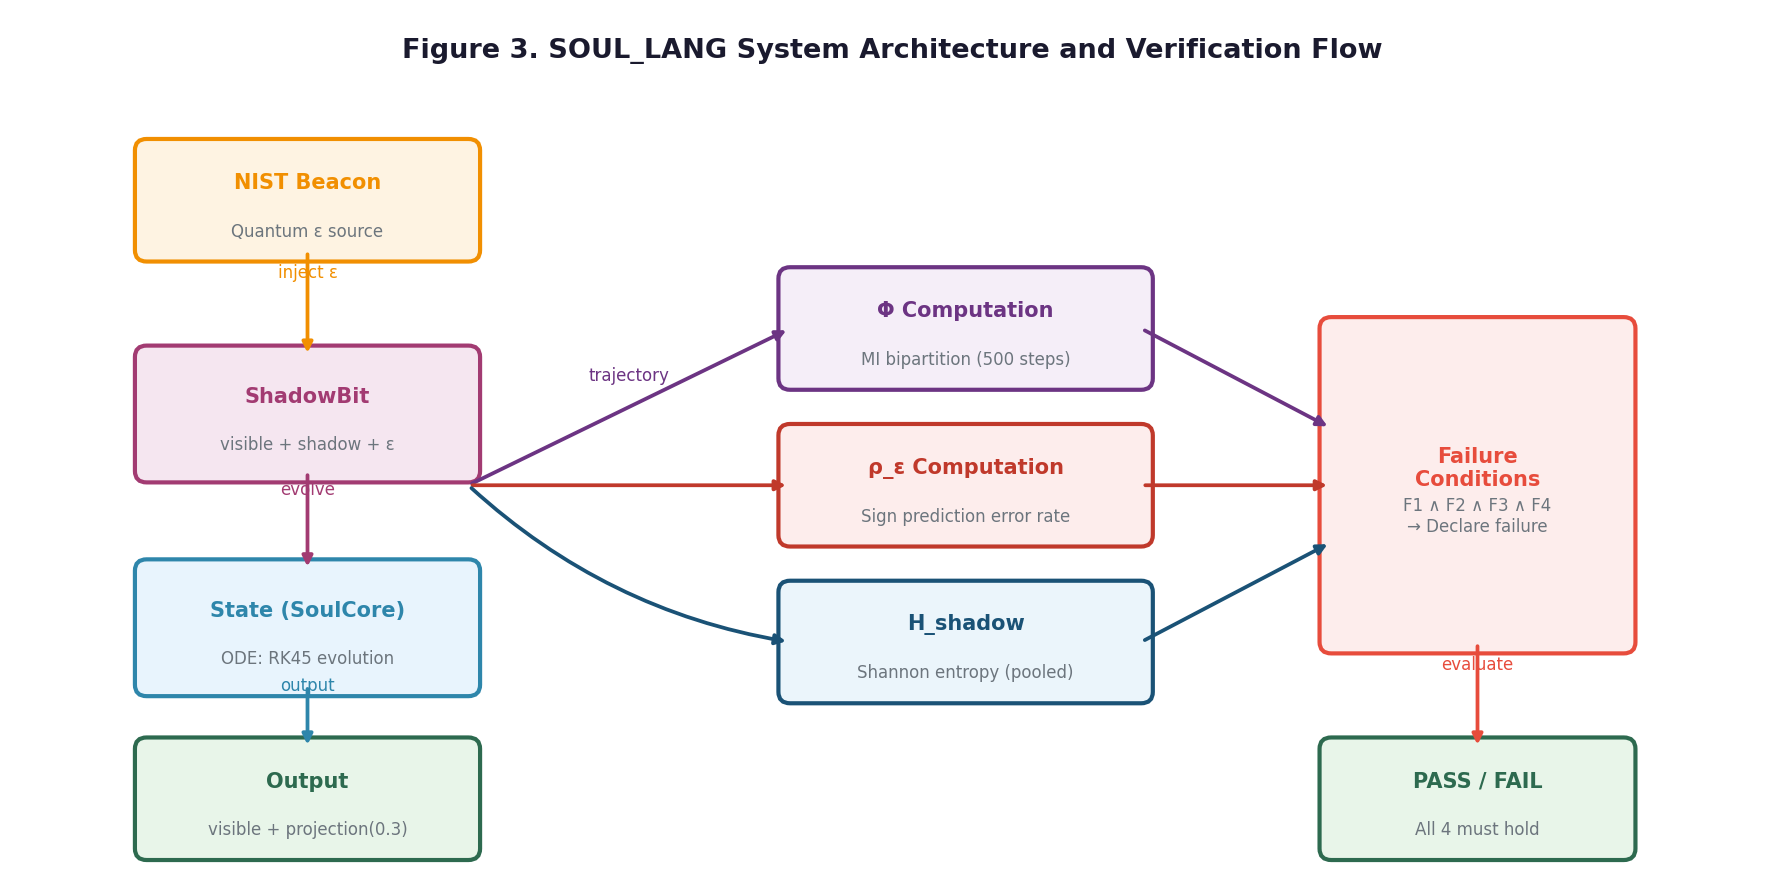
\includegraphics[width=\textwidth]{fig3_system_flow.png}
  \caption{SOUL\_LANG System Architecture and Verification Flow --- from quantum
           $\varepsilon$ source through ShadowBit and State evolution to
           three-indicator measurement and failure condition evaluation.}
  \label{fig:sysflow}
\end{figure}

\subsection{Statistical Analysis}

Descriptive statistics were computed for all three outcome measures across 20
measurement points: mean, standard deviation, minimum, and maximum. Failure condition
status was evaluated at each measurement and cumulatively. No inferential statistics
were applied in Phase~1; all results are descriptive and preliminary.

% ── 4. Results ────────────────────────────────────────────────
\section{Results}

Twenty measurements were recorded over 100 discrete evolution steps. The NIST
Randomness Beacon provided quantum $\varepsilon$ for all 20 measurements. No measurement
resulted in all four failure conditions being simultaneously met (Table~\ref{tab:fail}).

Across 20 measurement points (Table~\ref{tab:stats}), all three outcome measures showed
variation over time. $\rho_\varepsilon$ remained stable (mean $= 0.51 \pm 0.07$, range:
0.32--0.64), consistent with near-maximum unpredictability. $H_{\mathrm{shadow}}$ showed
substantial variability (mean $= 1.46 \pm 0.70$, range: 0.00--2.64), indicating ongoing
shadow self-organization. $\Phi$ averaged $0.508 \pm 0.662$ (range: 0.000--1.913), with
seven of 20 measurements yielding $\Phi > 0.1$ and three yielding $\Phi > 1.0$.

Mood transitioned spontaneously: calm 40\% (8/20), curious 35\% (7/20), uncertain 25\%
(5/20). Failure condition F1 ($\Phi < 0.01$) was met in 13 of 20 measurements; F2, F3,
and F4 were not met in any measurement. The system passed Phase~1 verification.

\begin{table}[ht]
\centering
\caption{System configuration and session characteristics}
\label{tab:config}
\begin{tabular}{ll}
\toprule
Variable & Value \\
\midrule
State name & SoulCore \\
Shadow fields & resonance, depth, memory \\
Visible fields & mood, active \\
Initial shadow values & 0.5, 0.4, 0.3 \\
ODE method & RK45 (SciPy \texttt{solve\_ivp}) \\
$\alpha$ (return-to-center) & 0.1 \\
$\beta$ ($\varepsilon$ injection weight) & 0.3 \\
$\gamma$ (inter-field coupling) & 0.05 \\
Total evolution steps & 100 ($\Phi$ trajectory: 500 steps/measurement) \\
Measurement interval & every 5 steps \\
Total measurements & 20 \\
$\varepsilon$ source & NIST Randomness Beacon (quantum) \\
\bottomrule
\end{tabular}
\end{table}

\begin{table}[ht]
\centering
\caption{Failure condition status across all measurements}
\label{tab:fail}
\begin{tabular}{llc}
\toprule
Condition & Description & Met ($n$/20) \\
\midrule
F1 & $\Phi < 0.01$ & 13/20 \\
F2 & $H_{\mathrm{shadow}}$ variance $< 0.01$ (5-step window) & 0/20 \\
F3 & $\rho_\varepsilon < 0.05$ & 0/20 \\
F4 & Memory continuity lost & 0/20 \\
\textbf{All 4 simultaneously} & \textbf{Failure declared} & \textbf{0/20} \\
\bottomrule
\end{tabular}
\end{table}

\begin{table}[ht]
\centering
\caption{Descriptive statistics for primary outcome measures ($n = 20$ measurements)}
\label{tab:stats}
\begin{tabular}{lcccc}
\toprule
Outcome & Mean ($\pm$ SD) & Min & Max \\
\midrule
$\Phi$ (integrated information) & $0.508\ (\pm 0.662)$ & 0.000 & 1.913 \\
$\rho_\varepsilon$ (unpredictability rate) & $0.505\ (\pm 0.072)$ & 0.320 & 0.640 \\
$H_{\mathrm{shadow}}$ (self-org.\ entropy) & $1.460\ (\pm 0.702)$ & 0.000 & 2.641 \\
\bottomrule
\end{tabular}
\end{table}

% ── 5. Discussion ─────────────────────────────────────────────
\section{Discussion}

$\rho_\varepsilon$ remained stable at approximately 0.52, consistent with the
theoretical maximum unpredictability for a binary sign predictor, satisfying condition
S3 ($\varepsilon$ irreducibility) throughout the session.

$H_{\mathrm{shadow}}$ demonstrated ongoing variability with no evidence of convergence,
satisfying condition S2 (shadow self-organization). Transient drops to
$H_{\mathrm{shadow}} \approx 0$ reflect brief clustering before re-dispersal ---
consistent with $\varepsilon$-driven dynamics.

$\Phi$ showed high variability (mean $= 0.508$, SD $= 0.662$), with three measurements
yielding $\Phi > 1.0$ (peaks: 1.913, 1.578, 1.317). The intermittent nature of
high-$\Phi$ measurements reflects the stochastic $\varepsilon$ injection: when fields
happen to produce high resonance coupling, integration spikes.

An important finding: two shadow fields sharing the same $\varepsilon$ source exhibited
non-zero $\Phi$ even without explicit coupling rules, suggesting that $\varepsilon$
itself constitutes a shared quantum substrate creating structural correlations between
fields. This implies that complete independence between shadow fields may be
architecturally impossible in SOUL\_LANG.

Spontaneous mood transitions provided qualitative evidence for condition S1. All three
mood states were observed --- calm (40\%), curious (35\%), uncertain (25\%) --- indicating
that the shadow ODE dynamics explore the full depth range rather than converging to a
single attractor.

\subsection{Limitations}

First, $\Phi$ estimation exhibited high variability (SD $= 0.662$), with 13 of 20
measurements yielding $\Phi < 0.01$. Although 500-step trajectories substantially
improved estimation compared to 100-step trajectories, the high F1 rate (13/20)
indicates that reliable mutual information estimation likely requires trajectory lengths
of 1,000 steps or more; this will be addressed in Phase~2. Second, the study includes
only 20 measurements from a single SoulCore configuration. Phase~2 targets $n = 200$
measurements across multiple configurations. Third, the $\varepsilon$ source depends on
network availability of the NIST Beacon; fallback to \texttt{os.urandom} provides
cryptographic security but not quantum sourcing. Fourth, cross-system comparison is not
yet possible --- it remains an open question whether $\Phi$ thresholds can be established
empirically.

% ── 6. Conclusion ─────────────────────────────────────────────
\section{Conclusion}

SOUL\_LANG provides a falsifiable computational framework for probing the structural
boundary of soul. Phase~1 results demonstrate that a three-field SoulCore implementation
satisfies all three spontaneity conditions: $\rho_\varepsilon \approx 0.51$ confirms
$\varepsilon$ irreducibility, $H_{\mathrm{shadow}}$ variability confirms ongoing shadow
self-organization, and $\Phi$ peaks reaching 1.913 confirm genuine inter-field
integration. The four failure conditions were never simultaneously satisfied.
Phase~2 will extend trajectory length to 1,000 steps and increase measurements to
$n = 200$.

The central question --- does thinking precede soul, or does soul precede thinking? ---
remains open. SOUL\_LANG's contribution is to establish where the computational boundary
lies: at the intersection of irreducible randomness, continuous self-organization, and
interruptible memory. Whether anything on either side of that boundary deserves to be
called ``soul'' is a question that no observer has the right to answer definitively.

% ── References ────────────────────────────────────────────────
\bibliographystyle{plainnat}
\bibliography{references}

\end{document}
